\documentclass{ctuthesis}
\usepackage{graphicx}
\usepackage{subfig}
\ctusetup{
	xdoctype = B,
	xfaculty = FCEyN,
	mainlanguage = czech,
	titlelanguage = czech,
	title-english = {Planting Uranium},
	title-czech = {Construcción e implementación de un sistema integral de 
	caracterización de filtros ópticos de interferencia de banda utilizados en 
	cámaras 
	hiperespectrales.},
	department-czech = {Departamento de Física},
	author = {Juan Reto Reynal},
	supervisor = {Prof. Dr. Hernán Grecco},
	supervisor-address = {Laboratorio de Electrónica Cuántica, DF, FCEyN, UBA.},
	month = 4,
	year = 2019,
}

\ctuprocess

\begin{abstract-english}
We develop \ldots
\end{abstract-english}

\begin{abstract-czech}
Rozvíjíme \ldots
\end{abstract-czech}

\begin{document}

\maketitle
\renewcommand{\chaptername}{Capítulo}
\renewcommand{\figurename}{Figura}
\chapter*{Plan de Tesis - Juan Reto Reynal}


\textsc{Título:} Construcción e implementación de un sistema integral de 
caracterización de filtros ópticos de interferencia de banda utilizados en 
cámaras 
hiperespectrales.


\hspace{-0.4cm}\textsc{Alumno:} Juan Reto Reynal L.U. 777/12.

\hspace{-0.4cm}\textsc{Director:} Dr. Hernán E. Grecco, Inv. Indep. CONICET, 
Prof. Adj. UBA.

\hspace{-0.4cm}\textsc{Lugar de trabajo:} LEC, Departamento de Física, FCEyN, UBA.


\section*{Objetivo general}

\hspace{0.5cm}La espectroscopía de imágenes hiperespectrales (HSI: 
\textit{Hyperspectral Spectroscopy Imaging}) combina la 
espectroscopía 
y la 
adquisición de 
	imágenes en dos dimensiones. Una imagen hiperespectral es generada a partir 
	de la colección y el procesamiento de imágenes de una muestra conformadas 
	por un gran número de bandas espectrales (típicamente entre 10 y 100), con 
	un ancho de banda muy estrecho de unos pocos nm, cubriendo de esta manera 
	de forma continua un rango espectral deseado. 

Este método brinda datos espectrales para cada pixel en el campo de 
visión\footnote{El campo de visión, en inglés \textit{field of view} (FOV), es 
el ángulo sólido a través del cual un sensor puede detectar la radiación 
electromagnética que se desee capturar.}. A partir de dichos 
datos se puede extraer información sobre la emisión, reflexión y absorción de 
la radiación electromagnética, que puede ser utilizada para determinar la 
composición química en diferentes áreas de la muestra.

Las cámaras de adquisición de imágenes hiperespectrales estándard utilizan 
redes de difracción o prismas como elementos dispersivos de la luz. La 
distancia requerida entre el sensor de detección y  el componente de difracción 
de la luz, 
hace que este tipo de cámaras sean muy grandes y muy pesadas, dos condiciones 
que por ejemplo en la industria satelital se quieren optimizar fuertemente ya 
que el costo de la puesta en órbita de los satélites es proporcional a su peso 
y a su tamaño. 
Estas cámaras suelen ser muy caras y muy sensibles a desalinearse 
debido a las 
condiciones mecánicas de su construcción. Además, requieren de una rendija 
para poder obtener una alta resolución espectral, lo que restringe 
significativamente la intensidad de la luz a detectar.

En respuesta a las numerosas desventajas de las cámaras estándard de imágenes 
hiperespectrales, aparecieron otro tipo de cámaras que utilizan filtros de 
interferencia de banda y que resultaron en un producto final robusto, compacto, 
de bajo costo y de muy buen rendimiento.


Hyperspectral imaging has been used in the past for applications such as air 
reconnaissance, satellite imaging and other markets that are not overly price 
sensitive. However, the emergence of alternative methods provides hyperspectral 
imaging with potential in volume markets and even consumer applications and 
products.
Precision farming, cancer detection, and food testing in supermarkets are just 
some examples of where the new approaches could be employed.

%semrock:
\hspace{0.5cm} Los filtros ópticos utilizados en la construcción de cámaras 
hiperespectrales y 
multiespectrales resultan fundamentales en aplicaciones como la microscopía de 
fluorescencia \cite{Grecco2016} y la espectroscopía de reflectancia 
utilizada para la toma de 
imágenes hiperespectrales de la superficie de la Tierra \cite{Hogg2008}.
 
 
 La capacidad de los filtros ópticos para transmitir ciertas longitudes de onda 
deseadas y bloquear el resto, resulta crítica para estas aplicaciones. Ahora 
bien, cuando el ancho de banda centrado en una cierta longitud de onda central 
que se desea transmitir es muy estrecho, las mediciones de las características 
espectrales y de transmisión de dichos filtros no suelen ser determinadas con 
precisión. Más aún, si los filtros son construidos especialmente por un 
proveedor (\textit{custom-made}) para una cierta aplicación específica, resulta 
fundamental su caracterización para decidir si incorporar o descartar dichos 
filtros a la carga útil de la aplicación en cuestión.

En una tesis de licenciatura anterior se co-desarrollo una camara 
hiperespectral ......

En el presente proyecto se propone desarrollar un sistema integral de 
caracterización de filtros de interferencia de banda con la capacidad de 
decidir si un filtro está apto o no para ser integrado a las cámaras 
hiperespectrales incorporadas en los satélites desarrollados por la empresa 
Satellogic.


%Optical filters play an important role in enabling applications such as 
%%%fluorescence
%microscopy and Raman spectroscopy. In these applications there are two 
%distinct types of
%beams: the illumination (or excitation) beam and the signal (or emission) 
%beam. 

%Not only are
%these beams spectrally distinct, but also they differ significantly in their 
%intensity – the signal
%beam can be a million times (or more) weaker than the illumination beam. 
%Therefore, the ability
%of filters to selectively transmit desired wavelengths of light while blocking 
%unwanted light is
%critical. The performance of such filters is determined by their spectral 
%characteristics, including
%transmission efficiency of the signal and attenuation (or blocking) of the 
%illumination light and
%undesirable emission wavelengths. In particular, often it is critical for 
%filters to transition from
%deep blocking to high transmission over a very short wavelength range, leading 
%to steep and
%deep spectral edges.
%However, due to limitations of standard metrology techniques, the
%measured spectral characteristics of thin-film interference filters are 
%frequently not determined
%accurately, especially when there are steep and deep edges.
%In this article we explore limitations to accurate filter spectrum 
%measurements with
%standard metrology techniques, and show how these limitations can be managed 
%by a better
%understanding of the limitations as well as more sophisticated measurements 
%when necessary.

\section*{Objetivos específicos del proyecto}
\begin{itemize}
	
	\item \texttt{Objetivo 0 - Abril:} Revisión del estado del arte.
	\item \texttt{Objetivo 1 - Mayo:} Armado de distintos setups de iluminación 
	o detección para distintas longitudes de onda para analizar los espectros 
	de transmisión de los filtros.
	\item \texttt{Objetivo 2 - Junio:} Armado de distintas configuraciones 
	experimentales controlando distintas formas de iluminar los filtros
	para poder encontrar los defectos.
	\item \texttt{Objetivo 3 - Agosto:} Construcción e implementación de un primer prototipo de un sistema integral que pueda decidir si un filtro está apto o no para ser integrado al satélite.
	\item \texttt{Objetivo 4 - Septiembre:} Establecer control de una de las cámaras de la empresa Satellogic para poder adquirir las
	imágenes. Procesar las imágenes tomadas haciendo HDR y búsqueda de características.
	\item \texttt{Objetivo 5 - Octubre:} Armado de un posible setup 
	experimental para poder caracterizar el filtro en su posición final
	en las cámaras de vuelo del satélite.
\end{itemize}
\section*{Introducción}

\hspace{0.5cm}La espectroscopia de imagen hiperespectral (HSI: 
\textit{Hyperspectral 
Spectroscopy Imaging}) está siendo desarrollada en numerosas aplicaciones, 
desde la industria satelital hasta la microscopía de células vivas.

Una imagen a color RGB convencional está compuesta por tres canales de 
imágenes (bandas): rojo 
($\sim$ 665nm), verde ($\sim$ 550nm) y azul ($\sim$ 470nm). Este tipo de 
imágenes permiten emular la percepción que el ojo humano tiene del color, pero 
no permiten la detección e identificación de distintos objetos sólidos y 
líquidos, menos 
aún determinar sus propiedades. Para ello 
es necesario obtener el espectro completo del objeto de estudio que es posible 
a partir de la captura de imágenes multiespectrales e hiperespectrales.

Las imágenes multiespectrales contienen un número acotado de bandas espectrales 
de hasta un par de decenas, con un gran ancho de banda (varias decenas de nm); 
mientras que las hiperespectrales están formadas por un gran número de bandas 
espectrales (de cientos a miles), con una resolución espectral muy estrecha, de 
unos pocos nm.

El esquema básico de una cámara hiperespectal de propósito general se muestra 
en la Figura \ref{fig:camsens}. Los filtros de interferencia de banda 
utilizados en este tipo de cámaras deben cumplir ciertos requisitos de calidad 
(no presentar rayones, ni marcas, etc) 
y ciertas características espectrales y de transmisión antes de ser 
incorporados a por ejemplo la carga útil de un satélite que va a ser puesto en 
órbita. En consecuencia, resulta fundamental caracterizar completamente dichos 
filtros antes de construir las cámaras de la aplicación de interés.

\begin{figure}[H]
	\centering
	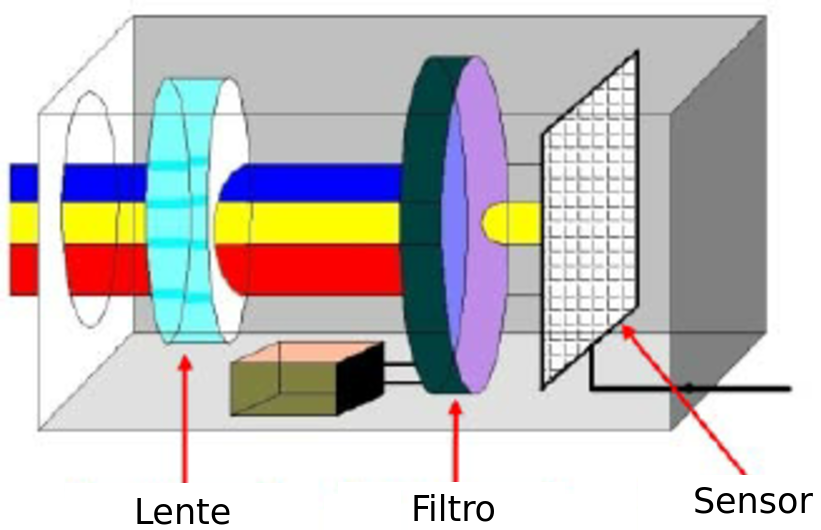
\includegraphics[scale=0.8]{Figs/plan_de_tesis/cam_sens.png}
	\caption{ Esquema de una cámara hiperespectral. El filtro absorbe el 
	espectro completo de la luz incidente salvo la banda espectral que el 
	usuario determina, por lo que sólo las longitudes de onda elegidas 
	atraviesan el filtro y son detectadas por el sensor. \cite{Martínez2016}}
	\label{fig:camsens}
\end{figure}



Debido a las limitaciones de las técnicas de 
medición estándard 
de los espectros de transmisión de los filtros ópticos donde se utilizan 
espectrómetros comerciales, las características de dichos 
filtros son determinadas generalmente de forma muy imprecisa, especialmente 
cuando el ancho de banda de transmisión centrado en una cierta de longitud de 
onda es muy estrecho (menos de una decena de nm para ciertas aplicaciones).


Como resultado de estas limitaciones, existen tres discrepancias fundamentales 
entre el espectro ''real''\footnote{El espectro ''real'' es 
	el espectro de diseño del filtro para el que fue especialmente construido.} 
	de 
un 
filtro y sus mediciones experimentales realizadas con 
espectrómetros comerciales (Ver Figura \ref{fig:obj1a})\cite{Semrock}. La 
primera discrepancia es el "redondeo" de características espectrales nítidas de 
los filtros. 
Esto se debe al ancho de banda no nulo del haz de la sonda del 
espectrómetro. 


La segunda discrepancia se debe al rango limitado de 
medición de la OD\footnote{La densidad óptica, OD (Optical Density), es un 
	parámetro útil para describir la transmisión de la luz a través de un 
	filtro 
	óptico con una transmisión extremedamente baja. Si T es la transmisión del 
	filtro, que varía entre 0 y 1, se define la densidad óptica como $OD = 
	-$log$_{10} (T)$.} del filtro, que es 
producto de la sensibilidad limitada del espectrómetro. Cuando un filtro 
tiene un valor de OD muy alto, OD $>$ 6, el detector debería medir una 
intensidad de la luz prácticamente nula pero el ruido óptico y electrónico 
propio del detector limita el nivel más bajo de intensidad que puede medir 
con precisión. De esta forma, se puede ver un ruido de piso debido al 
sensor indicando un cierto valor de OD que no coincide con el valor real 
del filtro.

\begin{figure}[h!]
	\centering
	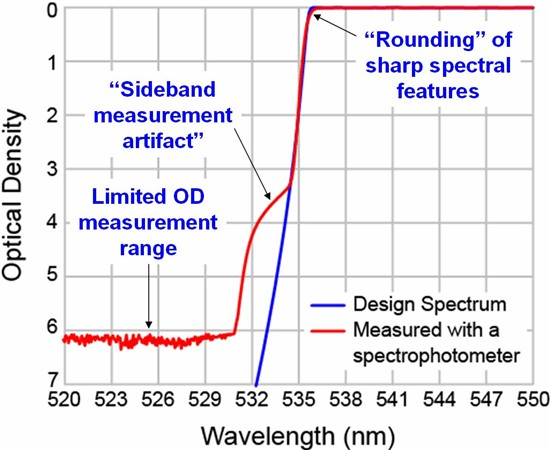
\includegraphics[scale=0.8]{Figs/plan_de_tesis/measurement_of_optical_filter.jpg}
	\caption{Discrepancias entre las mediciones experimentales con 
		espectrómetros 
		comerciales y el espectro ''real'' de un filtro óptico. Adaptado de 
		\cite{Semrock}.}
	\label{fig:obj1a}
\end{figure}

La tercera 
discrepancia es propia de las mediciones de transiciones muy 
pronunciadas. Esto surge 
por el hecho de que el 
haz de la sonda no es monocromático, sino que también tiene bandas 
laterales débiles de longitudes de onda fuera de su ancho de banda 
principal.




Ahora bien, dependiendo de la aplicación, las limitaciones en las mediciones 
del espectro de transmisión de los filtros pueden ser determinantes o no. En el 
presente proyecto se quiere determinar el arreglo experimental óptimo pero que 
sea compatible con los tiempos y costos de producción de la industria satelital.

\section*{Actividades asociadas al objetivo 1 - Mayo:}
\subsection*{ Armado de distintos setups de iluminación o detección para 
distintas longitudes de onda para analizar los espectros de transmisión de los 
filtros.}


\hspace{0.5cm}Las discrepancias de medición en espectrómetros convencionales 
causan 
importantes problemas al intentar evaluar el rendimiento del filtro para la 
aplicación prevista. 

La elección del instrumento de medición y la técnica 
empleada determinan la precisión de la medición del espectro de transmisión del 
filtro. Al mismo tiempo, determinan la duración y por ende también el costo de 
dichas mediciones, que deben ser compatibles con los tiempos que la industria 
requiere. Esto se puede ver con un ejemplo tomado de \cite{Semrock}. En la 
Figura \ref{fig:may_dists} se muestran cinco mediciones distintas de 
la densidad óptica de un filtro diseñado para bloquear longitudes de onda de 
532 nm con OD $>$ 6 y tener una transición a un estado de alta transmisión 
dentro del $0.5\%$ de la longitud de onda del láser utilizado para excitar la 
muestra, que es de 534.7nm.


\begin{figure}[H]
	\centering
	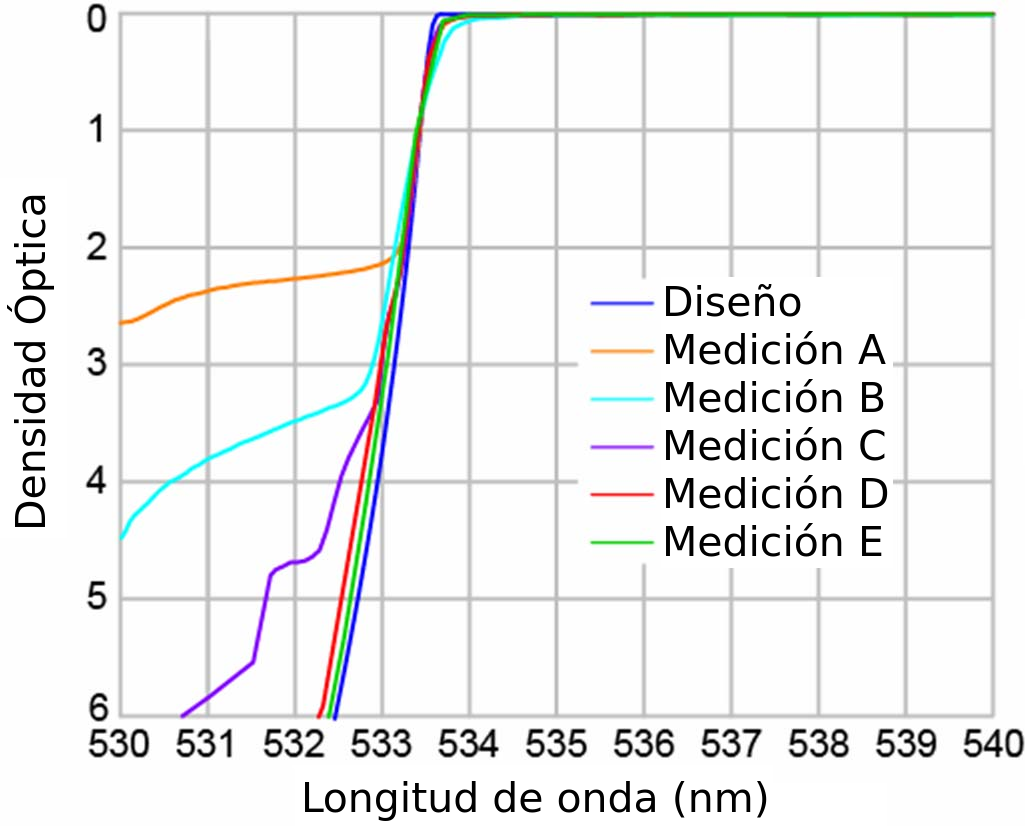
\includegraphics[scale=0.8]{Figs/plan_de_tesis/dists_meds.png}
	\caption{Distintas mediciones de la OD de un filtro LP03-532RE-
		25 RazorEdge de la empresa Semrock. Las mediciones fueron realizadas 
		utilizando tanto espectrómetros comerciales como \textit{custom-made} 
		de la emppresa con una variedad de arreglos experimentales que se 
		explican en el texto. Adaptado de 
		\cite{Semrock}.}
	\label{fig:may_dists}
\end{figure}

Las mediciones del método A fueron realizadas por un espectrómetro de diseño 
propio (\textit{custom-built}) de la empresa,  que tiene un tiempo de 
integración muy corto y una baja resolución, lo que resulta en una 
configuración 
experimental óptima para obtener mediciones de una gran cantidad de filtros de 
prueba. Este método es utilizado para determinar con precisión la longitud de 
onda a partir de la cual el filtro pasa a tener una alta transmisión, es decir, 
localiza la longitud de onda de la transición entre el estado de bloqueo y de 
transmisión del filtro, la longitud de onda de corte. De esta forma, se 
garantiza una cierta uniformidad en un lote de filtros a ser utilizado de una 
forma rápida y eficiente. Ahora bien, como se observa en el gráfico de la 
Figura \ref{fig:may_dists}, el método A posee una sensibilidad muy mala y una 
resolución muy baja, obteniéndose un piso de ruido mayor a OD 2.

El método B utiliza un espectrómetro comercial (Perkin Elmer
Lambda 900) cuyos inconvenientes fueron explicados a partir de las tres 
discrepancias en la Figura \ref{fig:obj1a}. Con este método no se puede 
asegurar que el filtro tenga un 0D $>$ 6 en los 532nm.


Los métodos C y D utilizan el mismo espectrómetro \textit{custom-built}	del 
método A, cuyo principio de funcionamiento básico se muestra en la Figura 
\ref{fig:med_prev}. La diferencia fundamental con el método B que utiliza un 
espectrómetro comercial es que las mediciones con el espectrómetro 
\textit{custom-built} realizan la detección con una cámara CMOS de bajo ruido, 
que consiste en un arreglo de detectores, por lo que puede medir en un rango 
muy grande de longitudes de onda simultáneamente. Este método permite en 
consecuencia obtener mediciones en un rango espectral muy grande, con una 
cierta resolución en un cierto tiempo de integración, de forma muy rápida.
El inconveniente fundamental de este método es que al utilizar una fuente de 
iluminación de banda ancha, si el filtro de prueba tuviera, por ejemplo, una 
autofluorescencia apreciable \cite{Shah2017}, podría interferir con una 
medición precisa de la transmisión de la muestra.


\begin{figure}[H]
	\centering
	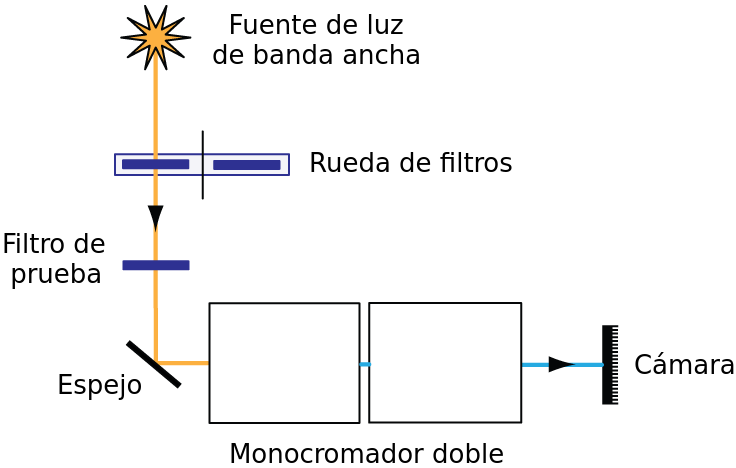
\includegraphics[scale=0.8]{Figs/plan_de_tesis/med_mets_prevs.png}
	\caption{Diseño básico de un espectrómetro \textit{custom-built} que 
	utiliza una fuente de iluminación de banda ancha y permite la recolección 
	de una 		amplia gama de
		longitudes de onda simultáneamente con un conjunto de detectores 
		situados en la cámara. Este 
		arreglo experimental permite una medición más rápida con un piso de 
		ruido y una resolución fijas. Adaptado de 
		\cite{Semrock}.}
	\label{fig:med_prev}
\end{figure}








\hspace{0.5cm}En ciertos filtros y aplicaciones, resulta de vital importancia 
el 
nivel de bloqueo de ciertos rangos de longitudes de onda pero no así la 
suavidad de la transición entre el bloqueo y la transmisión. Por ejemplo, en 
sistemas de 
imágenes de fluorescencia los espectros de absorción y emisión del fluróforo 
podrían estar lo suficientemente alejados como para que resulte fundamental que 
los filtros de banda de la señal de respuesta (de emisión) de la muestra tengan 
un bloqueo muy alto en la banda de la señal de excitación y así lograr una 
relación entre la señal y el ruido de adecuada proporción. 

Los filtros 
diseñados para estas aplicaciones podrían tener decenas de OD de bloqueo pero 
en 
la práctica incluso el más pequeño de los defectos físicos en los 
recubrimientos ópticos (\textit{coatings}) o en el montaje, así como el bajo 
nivel de control de luz parásita a nivel del sistema (**), puede limitar el 
bloqueo alcanzable a valores mucho menores que los del diseño original, en el 
rango de aproximadamente OD 6 a quizás 10.(forma indirecta de medir los scrath 
and dig!!**))) 

Dado que los espectrómetros 
comerciales estándard tienen una medición de OD de rango limitado debido al 
ruido de fondo del instrumento, se propone un arreglo experimental inicial para 
poder medir los niveles de bloqueo más altos con precisión como se muestra en 
la Figura \ref{fig:su} y que resulta compatible con la producción industrial 
deseada por su simplicidad.


\begin{figure}[h!]
	\centering
	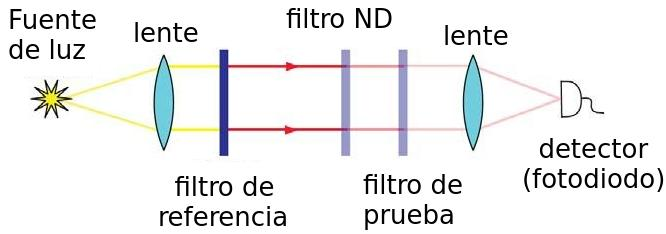
\includegraphics[scale=1.0]{Figs/plan_de_tesis/setup_u.jpeg}
	\caption{Arreglo experimental compatible con la producción industrial para 
	medir valores de 
	OD altos.}
	\label{fig:su}
\end{figure}

El método experimental de la Figura \ref{fig:su} se denomina 
\textit{complementary filter method}. Un haz de 
luz de banda ancha, de una lámpara QTH 
(\textit{Quartz-Tungsten Halogen}) ó de arco, aproximadamente colimado por una 
lente  es filtrado utilizando un filtro 
de referencia ampliamente bloqueador, que es esencialmente un filtro de banda 
con su banda de paso superpuesta a la región del espectro del filtro de prueba 
que se quiere analizar donde la medición de valores de OD altos son necesarios. 
La luz transmitida es enfocada con una lente convergente en un detector de bajo 
ruido capaz de medir niveles de intensidad de luz muy pequeños, como un 
fotodiodo de gran área con un circuito amplificador de bajo ruido ó un tubo 
fotomultiplicador (PMT).


Las mediciones se realizan de la siguiente manera. En primer lugar, se mide la 
intensidad de la señal en el detector con solo el filtro de referencia y un 
filtro calibrado de densidad neutra (ND) en la trayectoria de la luz. El filtro 
ND sirve para reducir el nivel de la intensidad de la luz en el detector en 
una cantidad calibrada de forma tal que el bias \footnote{El bias del 
detector es el valor medido por el instrumento cuando no hay ninguna fuente 
de luz incidiendo sobre él, es el valor de \textit{offset} que se le suma a 
cualquier 
medición.} del rango 
dinámico limitado alcanzable por el detector sea reducido para alcanzar los 
niveles de la señal que el detector va a ver cuando se coloquen los filtros de 
prueba. En particular, con un filtro ND 3, el rango dinámico del detector tiene 
que ser de $10^{6}$ para medir hasta un valor de OD 9 de bloqueo. En segundo 
lugar, se retira el filtro ND y se lo reemplaza por el filtro de prueba para 
realizar una nueva medición de la intensidad con el detector. El cociente entre 
las dos mediciones de intensidad de la luz es igual al valor de OD del filtro 
de prueba, en el rango espectral del filtro de referencia.


\section*{Actividades asociadas al objetivo 2 - Junio:}
\subsection*{Armado de distintos setups de iluminación 
	o detección para distintas longitudes de onda para analizar los espectros 
	de transmisión de los filtros.}

The actual blocking provided by a filter is determined not only by its designed 
spectrum, but
also by physical imperfections of the filter, such as pinholes generated during 
the thin-film
coating process, dirt and other surface defects, or flaws in the filter 
mounting. Pinholes can
allow light to pass through the filter unblocked – a single 10 $\mu$m pinhole 
(that 
penetrates
completely through the coating) limits the blocking of a 10 mm diameter beam to 
at most OD 6,
regardless of the designed level of blocking of the filter spectrum. Other 
surface and mounting
imperfections can cause scattered light that ''leaks'' through the filter due 
to 
a shift of the
spectrum to a region of high transmission for scattered light at high angles of 
incidence, or via unblocked paths near the edges or mounting. Therefore, it is 
important to evaluate the blocking
performance of filters after they have been fully manufactured into finished 
products.
%\section*{Actividades asociadas al objetivo 3 - Agosto:}
%\subsection*{Construcción e implementación de un primer prototipo de un 
%sistema 
%integral que pueda decidir si un filtro está apto o no para ser integrado al 
%satélite.}


%\section*{Actividades asociadas al objetivo 4 - Septiembre:}
%\subsection*{Establecer control de una de las cámaras de la empresa Satellogic 
%para poder adquirir las
%	imágenes. Procesar las imágenes tomadas haciendo HDR y búsqueda de 
%	características.}


%\section*{Actividades asociadas al objetivo 5 - Octubre:}
%\subsection*{Armado de un posible setup 
%	experimental para poder caracterizar el filtro en su posición final
%	en las cámaras de vuelo del satélite.}

\section*{Factibilidad}

\hspace{0.5cm}El lugar de trabajo donde el tesista va a desarrollar sus 
actividades es el 
Laboratorio de Electrónica Cuántica (LEC) del Departamento de Física de la 
Facultad de Ciencias Exactas y Naturales, UBA. El LEC cuenta con todas las 
instalaciones, infraestructura, instrumentos de medición y equipamiento 
necesarios para llevar a cabo la presente tesis. 

El director de la presente tesis es director del LEC y es experto en temas de 
óptica y fotofísica, áreas principales del proyecto. Además, tiene la 
experiencia de haber dirigido a una estudiante que realizó la tesis en conjunto 
con el LEC y la empresa Satellogic, resultando en una experiencia exitosa.

El tesista se encuentra cursando actualmente sus últimas dos materias de la 
carrera: 
Estructura de la Materia 4 e Instrumentación y Control.

El tesista junto a su director firmarán un NDA (Non-Disclosure Agreement) que 
le permitirán acceder a información importante para lograr el presente proyecto 
de tesis.**

\section*{Referencias}
1. [Hagen 2013] Nathan Hagen , Michael W. Kudenov. Review of snapshot spectral imaging technologies. Optical Engineering 52(9), 090901.

2. [Keshava 2003] Nirmal Keshava. A Survey of Spectral Unmixing Algorithms. Lincoln Laboratory Journal, Vol. 14, 1, 2003.

3. [Sellar 2005] R. G. Sellar and G. D. Boreman, “Comparison of relative signal-tonoise
ratios of different classes of imaging spectrometer,” Appl. Opt. 44(9), 1614–1624 (2005).

4. [Eismann 2012] M. T. Eismann, Hyperspectral Remote Sensing, SPIE Press, Bellingham, WA (2012).

5. [Harvey 2000] A. R. Harvey et al., “Technology options for imaging spectrometry,”
Proc. SPIE 4132, 13–24 (2000).

6. [Prieto 2008] X. Prieto-Blanco et al., “Optical configurations for imaging spectrometers,” Comput. Intell. Rem. Sens. 133, 1–25 (2008).

7. [Atherton 1981] P. D. Atherton et al., “Tunable Fabry-Perot filters,” Opt. Eng. 20(6),
806–814 (1981).

8. [Antila 2012] J. Antila et al., “Spectral imaging device based on a tuneable MEMS
Fabry-Perot interferometer,” Proc. SPIE 8374, 83740F (2012).

9. [Gupta 2008] N. Gupta, “Hyperspectral imager development at Army Research
Laboratory,” Proc. SPIE 6940, 69401P (2008).

10. [Poger 2001] S. Poger and E. Angelopoulou, “Multispectral sensors in computer
vision,” Technical Report CS 2001-3, Stevens Institute of Technology (2001).

11. [Potter 1972] A. E. Potter, “Multispectral imaging system,” U.S. Patent No. 3702735 (1972).

12. [Descour 1996] M. R. Descour, “The throughput advantage in imaging Fouriertransform spectrometers,” Proc. SPIE 2819, 285–290 (1996).

13. [Harvey 2004] A. R. Harvey and D. W. Fletcher-Holmes, “Birefringent Fourier-transform imaging spectrometer,” Opt. Express 12(22), 5368–5374 (2004).

14. [Mooney 1995] J. M. Mooney, “Angularly multiplexed spectral imager,” Proc. SPIE
2480, 65–77 (1995).

15. [Fernandez 2007] C. Fernandez et al., “Longwave infrared (LWIR) coded aperture
dispersive spectrometer,” Opt. Express 15(9), 5742–5753 (2007).

16. [Gehm 2008] M. E. Gehm et al., “High-throughput, multiplexed pushbroom hyperspectral microscopy,” Opt. Express 16(15), 11032–11043 (2008).

17. [Zimmermann 2005] Timo Zimmermann. Spectral Imaging and Linear Unmixing in Light Microscopy. Adv Biochem Engin/Biotechnol (2005) 95: 245– 265

18. Shima DT, Scales SJ, Kreis TE, Pepperkok R (1999) Curr Biol 9:821 

19. Ellenberg J, Lippincott-Schwartz J, Presley JF (1999) Trends Cell Biol 9:52

20. [Wouters 2001] Wouters FS, Verveer PJ, Bastiaens PI (2001) Trends Cell Biol 11:203
\chapter{Conclusion}

Lorep ipsum \cite{doe}


\renewcommand\bibname{Referencias Bibliográficas}
\begin{thebibliography}{1}

\bibitem{Mateen2018} Muhammad Mateen, Junhao Wen, Nasrullah and Muhammad Azeem 
Akbar, “The Role of Hyperspectral Imaging: A Literature Review” International 
Journal of Advanced Computer Science and Applications(IJACSA), 9(8), 2018. 
http://dx.doi.org/10.14569/IJACSA.2018.090808

\bibitem{Martínez2016} Martínez-Usó, Adolfo \& Pla, Filiberto \& Sotoca, José 
\& 
García-Sevilla, Pedro.(2008). From Narrow to Broad Band Design and Selection 
in Hyperspectral Images. 5112. 1091-1100. 
\href{https://www.researchgate.net/publication/221472272_From_Narrow_to_Broad_Band_Design_and_Selection_in_Hyperspectral_Images}{10.1007/978-3-540-69812-8\_109}.
 
 
 
\bibitem{Shah2017} Kamal G. Shah y Paul Yager.Wavelengths and Lifetimes of 
Paper Autofluorescence: A Simple Substrate Screening Process to Enhance the 
Sensitivity of Fluorescence-Based Assays in Paper. Anal. Chem. 2017,  89, 22, 
12023-12029. 2017.
 
\bibitem{Grecco2016} Hernán E. Grecco, Sarah Imtiaz y Eli Zamir. Multiplexed
imaging of intracellular protein networks. 2016.

\bibitem{Hogg2008} David W. Hogg y Dustin Lang. “Astronomical imaging: The
	theory of everything”. AIP Conference Proceedings. Vol. 1082.
	2008, págs. 331-338. \href{https://arxiv.org/pdf/0810.3851.pdf}{arXiv: 
	0810.3851.}

\bibitem{Semrock} Turan Erdogan y Prashant Prabhat. Semrock Technical Note 
Series: Measurement of 
Optical Filter Spectra. 

\end{thebibliography}

\end{document}

